\section*{Bilag}
\label{sec:bilag1}
\addcontentsline{toc}{section}{Bilag}
\renewcommand{\thesubsection}{\Alph{subsection}}

\subsection{Mail fra lampedesigner Erik}
\label{sec:mailErik}
Kære Mathias

Det er en meget komplex opgave i der er igang med, der er mange faktorer i spil når det handler om lys, både de fysiske, men ikke mindst de mentale. Jeg har i en del år arbejdet med lampedesign. og har derfor mest været optaget af armaturets/lampens skulpturelle udtryk, men da det jo er en lampe skal den selvfølgelig  også opfylde det belysningsmæssige behov. Jeg har arbejdet med mange lyskilder, lige fra glødepæren til det nyeste LED.I alle mine lamper er valg af lyskilde og placering sket på grundlag af test via prototyper. de fleste af mine lamper er prototyper. En af de mest krævende lamper, har været Gedserlampen, der har et specielt designet armatur, der kan sammensættes til forskellige højder. Gedserlampen er en reflektorlampe, og lyskilden er LED. det krævede utallige målinger, og det foregik såmænd kl 12 om natten, en tommestok på jorden og et luxmeter. Jeg vil nok foretrække prototype test, da de jo er tæt på virkeligheden, men måske kunne jeres software være en god hjælp i den indledende fase af et projekt? Du er velkommen til at kontakte mig igen hvis du tror jeg kan bidrage med noget.

Held og Lykke med projektet.

Venlig hilsen

Erik Mortensen

\subsection{Mail fra lampedesigner David fra IKEA Sverige}
\label{sec:mailDavid}
Hi! Apart from hand sketching and physical prototypes, we use the 3D modeling application Solid Works in IKEA of Sweden. And for renderings we use either the built in renderer, or photo works, which is also part of solid works.

Regards 

//David 

  On 9 October 2015 15:19:41 +08:00, Lasse Fribo Gadegaard <lgadeg15@student.aau.dk> wrote:
   
  Hello
   
   
  We are seven students from Aalborg university, that are writing a project on lamps and how they are design. And so we would like to ask you if you use any software to visualize your design, before they are made as a prototype or finished product. If you use any software feel free to tell us so we could research the software and get a better insight in the industry. I really hope you can help us. Thanks
   
   
  Regards,
  7 Students from Aalborg university

\subsection{Mail fra John Sørensen fra IKEA}
\label{sec:mailIKEA}
From: XX\newline
To: lasse-fribo@hotmail.com\newline
Subject: Lys og lamper - IKEA\newline
Date: Mon, 26 Oct 2015 15:25:23\newline

Hej Lasse.\newline

Tak for din mail\newline

Jeg har lidt svært ved at forstå, ved at læse vedhæftede spørgeskema, hvad jeres problemformulering er.\newline

Jeres spørgeskema har en ordlyd og formulering som kan opleves som negativt mod IKEAs produkter.\newline

Jeg forstår, at jeres projekt ikke handler om IKEAs produkter, men er en generel undersøgelse om lamper og lys. Udfordringen er at vores kunder vil læse spørgsmålene og relatere det til IKEA, da I henvender jer til vore kunder i varehuset. Da spørgsmålene handler om utilfredshed, er vi bekymrede for denne kobling. På den baggrund, kan vi desværre ikke tilbyde jer at gennemføre undersøgelsen her i varehuset.\newline

Med venlig hilsen\newline
John Kristian Sørensen\newline
Store Manager\newline
IKEA Aalborg A/S\newline
\noindent\makebox[\linewidth]{\rule{\paperwidth}{0.4pt}}
From: lasse fribo gadegaard\newline
Sent: 30. oktober 2015 14:04\newline
To: John Sørensen\newline
Subject: RE: Lys og lamper - IKEA\newline

Hej igen,\newline

Jeg vedhæfter vores spørgeskema og vi vil meget gerne komme enten mandag, tirsdag efter kl 12 eller torsdag efter kl 14. \newline

Venlig hilsen\newline
Lasse Fribo Gadegaard og resten af gruppe B2-28
\noindent\makebox[\linewidth]{\rule{\paperwidth}{0.4pt}}
From: XX\newline
To: lasse-fribo@hotmail.com\newline
Subject: Lys og lamper - IKEA\newline
Date: Mon, 26 Oct 2015 12:43:25\newline

Hej Lasse.\newline

Som aftalt sender jeg mine kontaktoplysninger.\newline

I må gerne sende mig de spørgsmål I ønsker at stille vore kunder og forslag til dato I kommer til IKEA.\newline

Ønsker dig en god dag.\newline

Med venlig hilsen\newline
John Kristian Sørensen\newline
Store Manager\newline
IKEA Aalborg A/S\newline

\subsection{Mail fra belysningskonsulent}
\label{sec:mailbelysning}
Fra: XX \newline
Sendt: 6. november 2015 13:36 \newline
Til: Lasse Fribo Gadegaard\newline
Emne: SV: Semesterprojekt om lamper - AAU\newline
Hej
 
Det at se en lampe i 3D gør ikke at man ser lyset. Nogle af vores producenter laver allerede 3D modeller af deres lamper og endda sådan at man kan se lampen med lys i. Jeg har lige vedhæftet Artemides udgave af fremgangsmåden.

Men derfra til at se hvordan lyset er i et konkret rum hvor farver, højde mv. har indflydelse på lyset gør at det bliver en ekstrem kompleks størrelse der kræver komplicerede belysningsberegningsprogrammer som f.eks. DIALux. Lysberegning handler primært om lysmængde og ikke om lyseffekt.

Kunder har svært ved at forstå er hvilken lyseffekt lampen giver. Det er jo to-siddet. Dels vil de se hvordan lampen ser ud i rummet og dels vil de se hvordan lyseffekten er. Første del klarer flere producenter. Hvis man så bagefter at man har sat lampen ind som 3D model burde man lave et lag over billedet hvor producenten så har taget et billede af et rum hvor man kan se skygger mv. Eks Tom Dixon. Det er det jo ikke lampe man køber men ofte lyseffekt og lampe handler jo om at forme lyset og lave skygger. At sætte en Tom Dixon lampe ind i et rum gør ikke at du kan se skyggerne.

Det er blevet en kompliceret proces at producere en lampe ift. EU lovgivning i dag så jeg har svært ved at se at producenterne vil koste endnu flere penge til produkter til privatmarkedet som måske kun køber en lampe til 3000 kr. som ofte kun interesserer sig for den laveste pris og ikke den bedste service og rådgivning. Så producenters incitament til ligge investeringer hos privatkunder er meget begrænset. Mange laver end ikke et fritskravet billede af deres lampe. Og igen Tom Dixon anvender en klar halogenlyskilde. Hvis du sætter en klar kultrådslyskilde hvor filamentet er længere giver forsat skygger men på en blødere måde da lyset er delt ud på en større overflade. Hvis du sætter en mat lyskilde i forsvinder skyggerne næsten helt. Pludselig er løsningen bare komplekst og når en producent så har 4000 varenumre. Samme lyskilder laves så i 3 farvetemperaturer. Med vores adgang til varesortiment giver det 2 mio. billeder dokumenter som skal indhentes. Så er vi der hvor det begynder ikke at hænge sammen tidsmæssigt når nethandlen handler om at være først ift. googlesøgninger mv. Hvem har lyst til at give bedste rådgivning ift. lyseffekter hvis man ender på side 20 når folk søger på google?  

Løsningsforslag modtages derfor med kyshånd da kompleksitet er desværre nem at se. 

I må selvfølgelig også gerne vores udtagelser.  

Med venlig hilsen / best regards

XX\newline
Belysninskonsulent

\noindent\makebox[\linewidth]{\rule{\paperwidth}{0.4pt}}

Fra: Lasse Fribo Gadegaard [mailto:lgadeg15@student.aau.dk] \newline
Sendt: 6. november 2015 11:19\newline
Til: XX\newline
Emne: SV: Semesterprojekt om lamper - AAU

Hej 
 
Vi er meget glade for at I vil bidrage til projektet. Indtil videre har vi analyseret problemet: 
Forbrugeren kan ikke visualisere, hvordan lyset udbreder sig fra en lampe uden at købe og installere lampen. 

I problemanalysen har vi undersøgt interessenter, begreber, placering og teknologier til problemet. 

Ud fra dette har vi valgt at fokusere på e-butikker, der sælger indendørs lamper til brug i erhverv eller private hjem. 

Vi har netop udarbejdet den endelige problemformulering, hvor udkastet lyder som følgende:
Hvordan kan man lave et værktøj til e-butikker som vha. raytracing*, visualiserer belysningen fra indendørs lamper for kunderne? 

* En teknik til at simulere lys og lave et billede af en 3D-model. 

Vi skal nu til at udvikle en løsning til problemet, og hertil har vi lavet en simpel skitse (Se vedlagt billede) af den ide vi har på nuværende tidspunkt. 
 
Som vist på skitsen, er ideen at lave et produkt som gør det muligt for kunderne at se nogle lamper og deres belysning i et interaktivt 3D-billede på e-butikken. 

Vi tænker at forbrugeren skal kunne gøre følgende: \newline
 - Vende og dreje billede, så de kan se lampen og belysningen fra flere vinkler. \newline
 - Se lampen med forskellige pærer (evt. angive farvetemperatur i Kelvin) \newline
 - Skifte den kontekst som lampen visualiseres i (f.eks. forskellige rum/møbler)

Pga. tidsbegrænsning forventer vi ikke at lave hele løsning, som produkt, men blot implementere de mest studierelevante dele. 

Dog skal vi stadigvæk præsenterer en færdig løsning i rapporten. 

Det vi nu ønsker jeres respons på, er følgende
 - Jeres tanker omkring ideen, som løsning på problemet.\newline
 - Forslag og ønsker til forbedringer af ideen. \newline
 - Jeres accept til, at vi i rapporten må inddrage jeres udtagelser anonymt.

Med venlig hilsen,\newline
Lasse Gadegaard
 
På vegne af \newline
Gruppe B2-28\newline
Software, AAU
 
\noindent\makebox[\linewidth]{\rule{\paperwidth}{0.4pt}}

Fra: XX \newline
Sendt: 5. november 2015 15:43\newline
Til: Lasse Fribo Gadegaard\newline
Emne: SV: Semesterprojekt om lamper - AAU\newline
Hej Lasse

Det lyder til at være et meget spændende projekt.
 
Som primær detailforretning med projektafdeling lever vi af konsulentarbejde ved at give rådgivning omkring hvordan lys forandre sig ift. til lofthøjde, farver, armatur, lyskilde foruden at der er en subjektiv mening om hvad godt lys er.

Der er overraskende mange der gerne vil se lyset inden de køber lamper. Man kan dog undre sig ovre at samme kunde køber både køleskabe, vaskemaskiner mv. uden at stille krav til at prøve tingene før de køber varerne selv om disse produkter koster lige så meget som de lamper vi sælger. Kunder har åbenbart et specielt forhold til lys. 

Har i allerede valgt teori, metode og empiri? 

Jeg tror godt vi kan hjælpe jer. Eneste krav er at data herfra bliver anonymiseret og vi får et eksemplar af opgaven når den er skrevet.

God dag

Med venlig hilsen / best regards\newline
XX\newline
Belysningskonsulent

\noindent\makebox[\linewidth]{\rule{\paperwidth}{0.4pt}}

Fra: Lasse Fribo Gadegaard [mailto:lgadeg15@student.aau.dk] \newline
Sendt: 5. november 2015 15:06\newline
Til: XX\newline
Emne: Semesterprojekt om lamper - AAU
 
Hej XX
 
Vi er en gruppe på Aalborg Universitet, som er i gang med et projekt om visualisering af lamper.
 
Vi arbejder med følgende problemstilling:
"Forbrugeren kan ikke visualisere, hvordan lyset udbreder sig fra en lampe uden at købe og installere lampen." 

Vi har fokus på e-handel, og ønsker at tilbyde e-butikken et værktøj som gør det nemmere for kunderne at visualisere, hvordan lyset breder sig ud fra en lampe (f.eks. hvilke skygger, mønstre og farver som lampen udsender). 

Derfor søger vi nu e-butikker, som ønsker at bidrage med viden og informationer omkring e-handel med lamper.  

Hvis I er interesserede i at medvirke i projektet, så skriv venligst tilbage på mail: lgadeg15@student.aau.dk 

Med venlig hilsen,\newline
Lasse Gadegaard\newline
På vegne af\newline
Gruppe B2-28\newline
AAU, Software


\subsection{Spørgeskema}
\label{sec:skema}
\begin{figure}[H]
    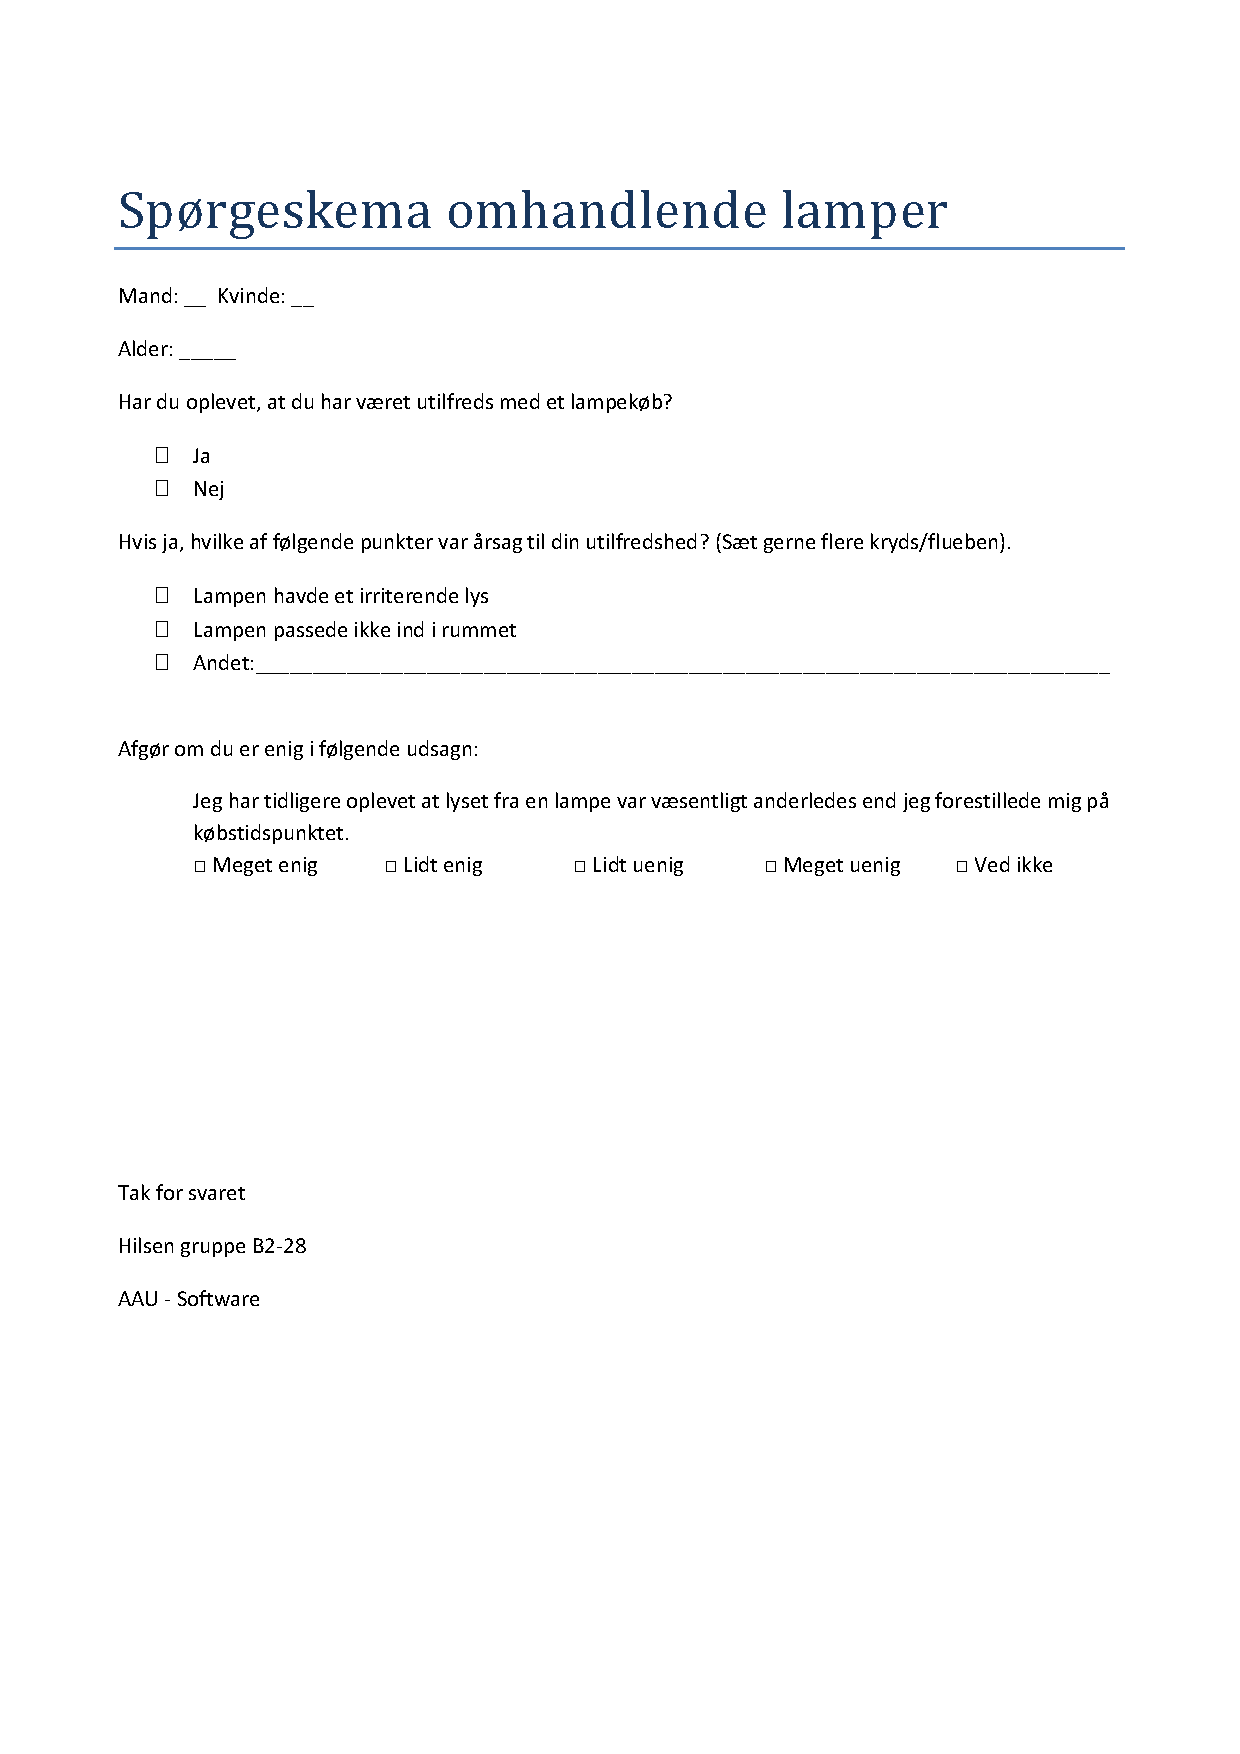
\includegraphics[height=15cm]{sporgeskema}
\end{figure}
